%In this section, we will discuss generalizable trends of factors contributing to a community's accessibility risk, which offer insight into possible opportunities for risk mitigation. 
%
%\subsection{Trends by car ownership class}
%\label{sec:carEquity}
%From Section~\ref{sec:accAll}, we notice that the ratio of cars to the number of people who work in a household is strongly correlated with accessibility risk; a higher ratio corresponds to higher expected decreases in accessibility. This result could stem from a few causes. 
%
%First, we have seen that households living in communities, such as Danville, CA, that on average take longer trips, are at greater risk. Thus, we might expect households at greater risk, i.e., households with more cars, to take longer trips. This is indeed the case (Figure~\ref{fig:lengthIncomeBars}{(b)}). However, as suggested in Section~\ref{sec:accSF}, trip length is not fully predictive. In fact, there is only a weak trend between average trip length for a TAZ before any earthquake and the predicted impact on accessibility (Figure~\ref{fig:accLength}).
%
%Instead, we predict that there are other latent variables correlated with car ownership. For example, the geographic distribution of people without cars varies. Additionally, in Section~\ref{sec:acctravelshift}, we will further explore the correlation between the percentage of car-based trips and accessibility risk. We will show that TAZs with fewer car-based trips, tend to have lower risk of accessibility losses.
%
%
%\begin{figure}
%\centering
%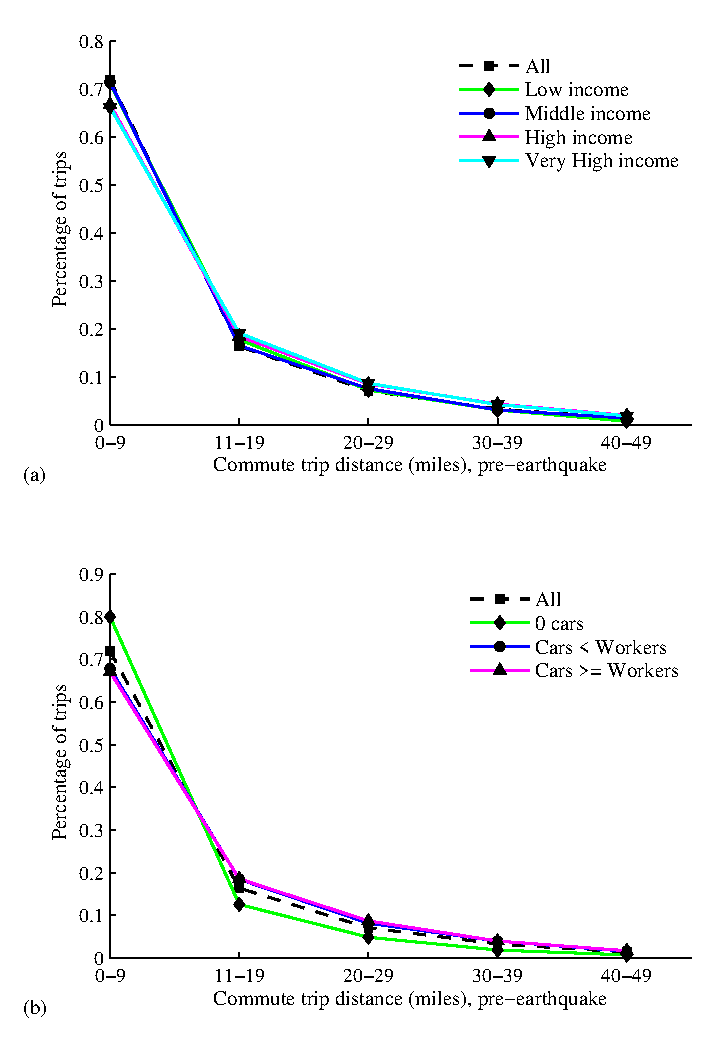
\includegraphics[width=5in]{../FIGS/equity_trip_distance_income_cars_to_and_from_work.eps} 
%\caption{Distributions of commute trip length in 10-mile intervals  by a) income class segment, and b) car ownership segment,  (pre-earthquake)}
%\label{fig:lengthIncomeBars}
%\end{figure}
%
%%\subsection{Impact of trip length}
%%
%\begin{figure}
%\centering
%\includegraphics[width=6in]{../FIGS/equity_accLength.eps} 
%\caption{Trip length (pre-earthquake) versus change in total accessibility per person per day}
%\label{fig:accLength}
%\end{figure}
%
%
%
%
%\subsection{Trends by income class}
%Controlling for car ownership, we see a fairly equitable distribution of risk across income class segments.  For example, by looking at households with fewer workers than cars, the variation from TAZ to TAZ is significantly more striking than the difference across income segments (Figure~\ref{fig:acc_by_segment}{(b,e,h,k)}). Similarly, while trip lengths are slightly longer for higher income households, the differences are subtle (Figure~\ref{fig:lengthIncomeBars}{(a)}).
%
%
%Thus, for a given TAZ, the differences across incomes are not that great. However, there is an unequal geographic distribution of wealth in the San Francisco Bay Area. Because of this, when we aggregate accessibility risk across TAZs, we see that accessibility risk rises with increasing household income  (Figure~\ref{fig:acc_by_TAZ_and_income}{(b)}). Therefore, even though the poor are generally the most vulnerable to climatological and geophysical hazards and disasters, such as hurricanes, floods and earthquakes~\cite{fothergill_race_1999},  wealthier households in the San Francisco Bay area are more vulnerable than the other income groups to earthquake-related accessibility risk.
%
%%\begin{figure}
%%\centering
%%\includegraphics[width=6in]{../FIGS/equity_accCCDF_by_Income.eps} 
%%\caption{Trip length (pre-earthquake) versus change in total accessibility (households with the number of cars less than the number of workers) }
%%\label{fig:equity_accCCDF_by_Income}
%%\end{figure}
%
%
%
%%look above for subfigure b that has length vs. income segment
%
%%but note that income is tied to car ownership...
%
%
%
%
%
%%\begin{figure}
%%\centering
%%\includegraphics[width=\textwidth]{../FIGS/equity_dataset_count_matrix_hh.eps} 
%%\caption{Household-by-household distribution of car ownership by income class (as percentage of total number of households)}
%%\label{fig:car}
%%\end{figure}
%\begin{figure}[h]
%\centering
%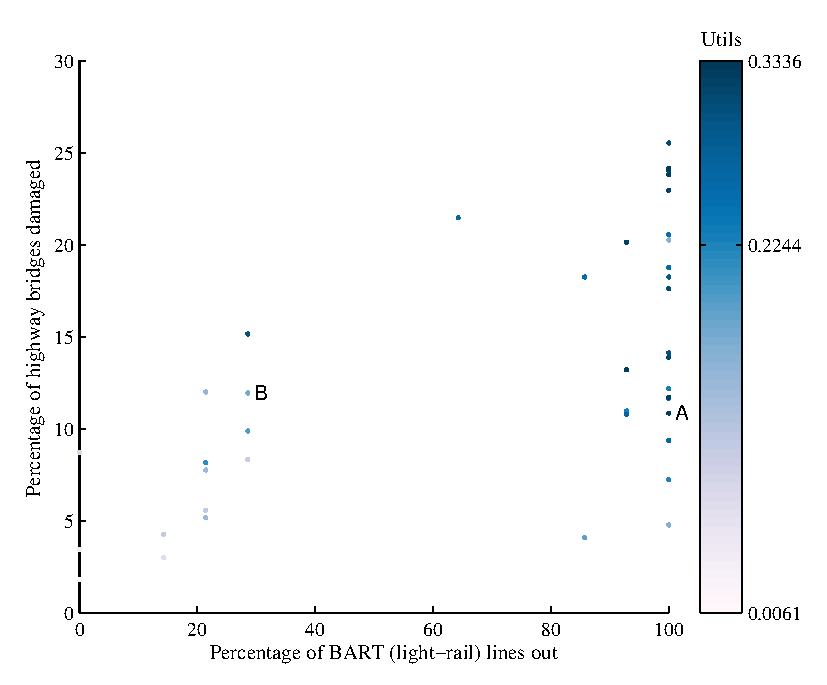
\includegraphics[width=6in]{../FIGS/equity_bart_bridges_acc.eps} 
%\caption{Percentage of BART (heavy-rail) lines not operational versus percentage of highway bridges damaged for each of the 40 events. The values are color-coded by the average loss in accessibility per day per person over all TAZs (for the market segment of households with the number of cars less than the number of workers). Two events discussed in this section are marked by the letters A and B.}
%\label{fig:bartBri}
%\end{figure}
%
%\subsection{Impact of travel mode shifts and regional variations in travel mode patterns on accessibility risk} \label{sec:acctravelshift}

%\subsection{Impact to accessibility risk of both travel mode shifts and regional variations in travel mode patterns} \label{sec:acctravelshift}
%Two key factors related to the resilience of a community to transportation network damage are the post-earthquake functionality of the relevant transit systems, and  how conducive a community is for trips by bike or by foot. 

%In this section, we will compare patterns of transit system damage with patterns of travel mode shifts after earthquake events, and then discuss the corresponding trends in accessibility impact. Then, we will examine the correlation between a community's walkability and bike friendliness, as measured by the percentage of total trips made by those travel modes, and the expected losses in accessibility by community. 





\begin{figure}[htb]
\centering
\includegraphics[width=4in]{FIGS/equity_bart_bridges_acc3vJWBv4.eps} 
\caption{Percentage of BART lines not operational versus percentage of highway bridges damaged, where each data point corresponds to one earthquake simulation. The points are color-coded by the average loss in accessibility per day per person over all TAZs for households with the fewer cars than workers.}
\label{fig:bartBri}
\end{figure}



First, we compare patterns of transit system damage with patterns of travel mode shifts after earthquake events. Over all the simulated events, taking a weighted average by the annual occurrence rate of each event, we see a 25\% reduction in transit ridership after an earthquake. The heavy rail systems (BART and Caltrain) are not fully operational in most of the forty simulated events (Table~\ref{tab:transit}), and these have heavy ridership. The light rail systems (VTA and Muni) also suffer losses in many events (Table~\ref{tab:transit}). %As detailed in~\cite{miller_seismic_2014}, with regards to the other transit systems, trans-bay and cross-county bus lines were suspended in the forty events and the baseline case; main local buses are modeled as operational, although with possible delays; and ferries are modeled as operational.
% in only 13 out of the 40 earthquake events, are more than 50\% of the BART lines running, with similar trends for other transit systems. 
Some of the pre-earthquake transit trips do not take place at all in the post-earthquake simulations, and some switch to other modes (foot, car, and bike), causing small average increases in the number of trips taken by other modes. One exception to this trend is the M6.35 Great Valley, Pittsburg-Kirby Hills Fault earthquake event, illustrated in Figure~\ref{fig:scen_acc}{e and~\ref{fig:scen_acc}{f}. In this event, there were no line closures on the four major transit systems listed in Table~\ref{tab:transit}. There were, however, some bridge closures on the highways, resulting in a slight increase in transit ridership and also in trips by foot.

\begin{table*}
\caption{Number of the 40 earthquake realizations in which for major transit networks have a specified level of functionality. Functionality is measured by the percentage of lines that are operational in a given realization. }
\centering
\begin{tabular}{c||c|c|c|c}
\textbf{Functionality}           & \textbf{BART} & \textbf{Caltrain} & \textbf{Muni Light Rail} & \textbf{VTA Light Rail}  \\
\hline
Full & 3 & 13 & 25 & 9\\
50-99\%  & 10 & 0 & 15 & 0\\
1-49\%  & 8 & 0 & 0 & 0\\
None & 19 & 27 & 0 & 31\\
\end{tabular}
\label{tab:transit}
\end{table*}


%The result is approximately a 1.3????\% change in travel mode. This is roughly consistent with the 14\% change in travel mode estimated after the 1994 Northridge earthquake~\cite{gordon_transport-related_1998}.

In general, accessibility impact grows with increasing number of damaged transit lines, particularly in combination with high numbers of damaged bridges (Figure~\ref{fig:bartBri}). Individual network simulations also suggest that transit is a key contributor to accessibility risk. For example, the M6.85 Hayward Rogers-Creek and the M7.45 Northern San Andreas Fault events from Figure~\ref{fig:scen_acc} both have around 11\% of bridges damaged. These events are labeled in Figure~\ref{fig:bartBri}, which indicates that the Hayward Rogers-Creek event has significantly higher transit network damage and accessibility loss. The Northern San Andreas event had 10 of the 14 BART lines and all Muni lines operational, whereas the Hayward Rogers-Creek event had no BART lines and 5 of the 8 Muni lines operational (Caltrain and VTA were not operational in either simulation).  
Moreover, the differences in accessibility results could not have been predicted from simpler models focusing on bridge portfolio losses, because the percent of damaged bridges was about the same, and the San Andreas event actually corresponded to a greater increase in fixed-demand travel time when modeled using a much simpler traffic model.

%In general, accessibility impact grows with increasing number of damaged transit lines, particularly in combination with high numbers of damaged bridges (Figure~\ref{fig:bartBri}). The results do not conclusively show that transit is a key contributor to accessibility risk, but based on individual examples, the data suggests this conclusion. For example, the  M7.05 Hayward Rogers-Creek Fault event discussed above and the M7.45 Northern San Andreas Fault event both have a similar number of damaged bridges; these are noted by points A and B respectively in Figure~\ref{fig:bartBri}. However, this Hayward Rogers-Creek event has significantly higher accessibility impact. Similarly, the transit impact was different. This Northern San Andreas event had only 4 of the 14 BART lines, all Caltrain and all VTA Light Rail lines not operational, whereas this Hayward Rogers-Creek event had all 14 of the 14 BART lines, all Caltrain, all VTA Light Rail and 3 of the 8 Muni light rail lines not operational. Thus, the transit lines were significantly differently impacted. Furthermore, the accessibility results could not have been predicted from the efficient transportation model introduced in  Section~\ref{sec:caseMet}.

% For example, the xxxx event and the xxxx event have similar number of damaged bridges and a similar travel time predicted from the efficient fixed-demand model. However, the xxxx event has significantly higher accessibility impact. Similarly, the transit impact was different. The xxxx event had xxx and the xxxx event had xxxx.

Next, we examine the correlation between a community's walkability, as measured by the percentage of total trips made by that travel mode, and its expected decrease in accessibility. Figure~\ref{fig:walkingVsAcc} shows that communities with a high percentage of pre-earthquake trips on foot have a lower average decrease in accessibility. This result corroborates the specific example of the San Francisco Financial District discussed in Section~\ref{sec:accSF}. Furthermore,  on average, the number of by-foot trips increases after the earthquake events where road congestion worsens. This model result is consistent with the observations after the 1995 Kobe earthquake, in which many commuters switched to walking and biking in the weeks after the earthquake~\cite{gordon_transport-related_1998}. This suggests that communities with greater walkability are also more resilient to earthquake-related accessibility risk. 

\begin{figure}[htb]
\centering
\includegraphics[width=4in]{FIGS/equity_footVsAccv3.eps} 
\caption{Percentage of pre-earthquake trips taken by foot versus expected decrease in accessibility among households with fewer cars than workers, for all TAZs in the study area. Each dot represents data from one TAZ, and red dots highlight the data points for the three case study communities.}
\label{fig:walkingVsAcc}
\end{figure}


%\subsection{Limitations}